\section{Results}

\begin{figure*}[h]
  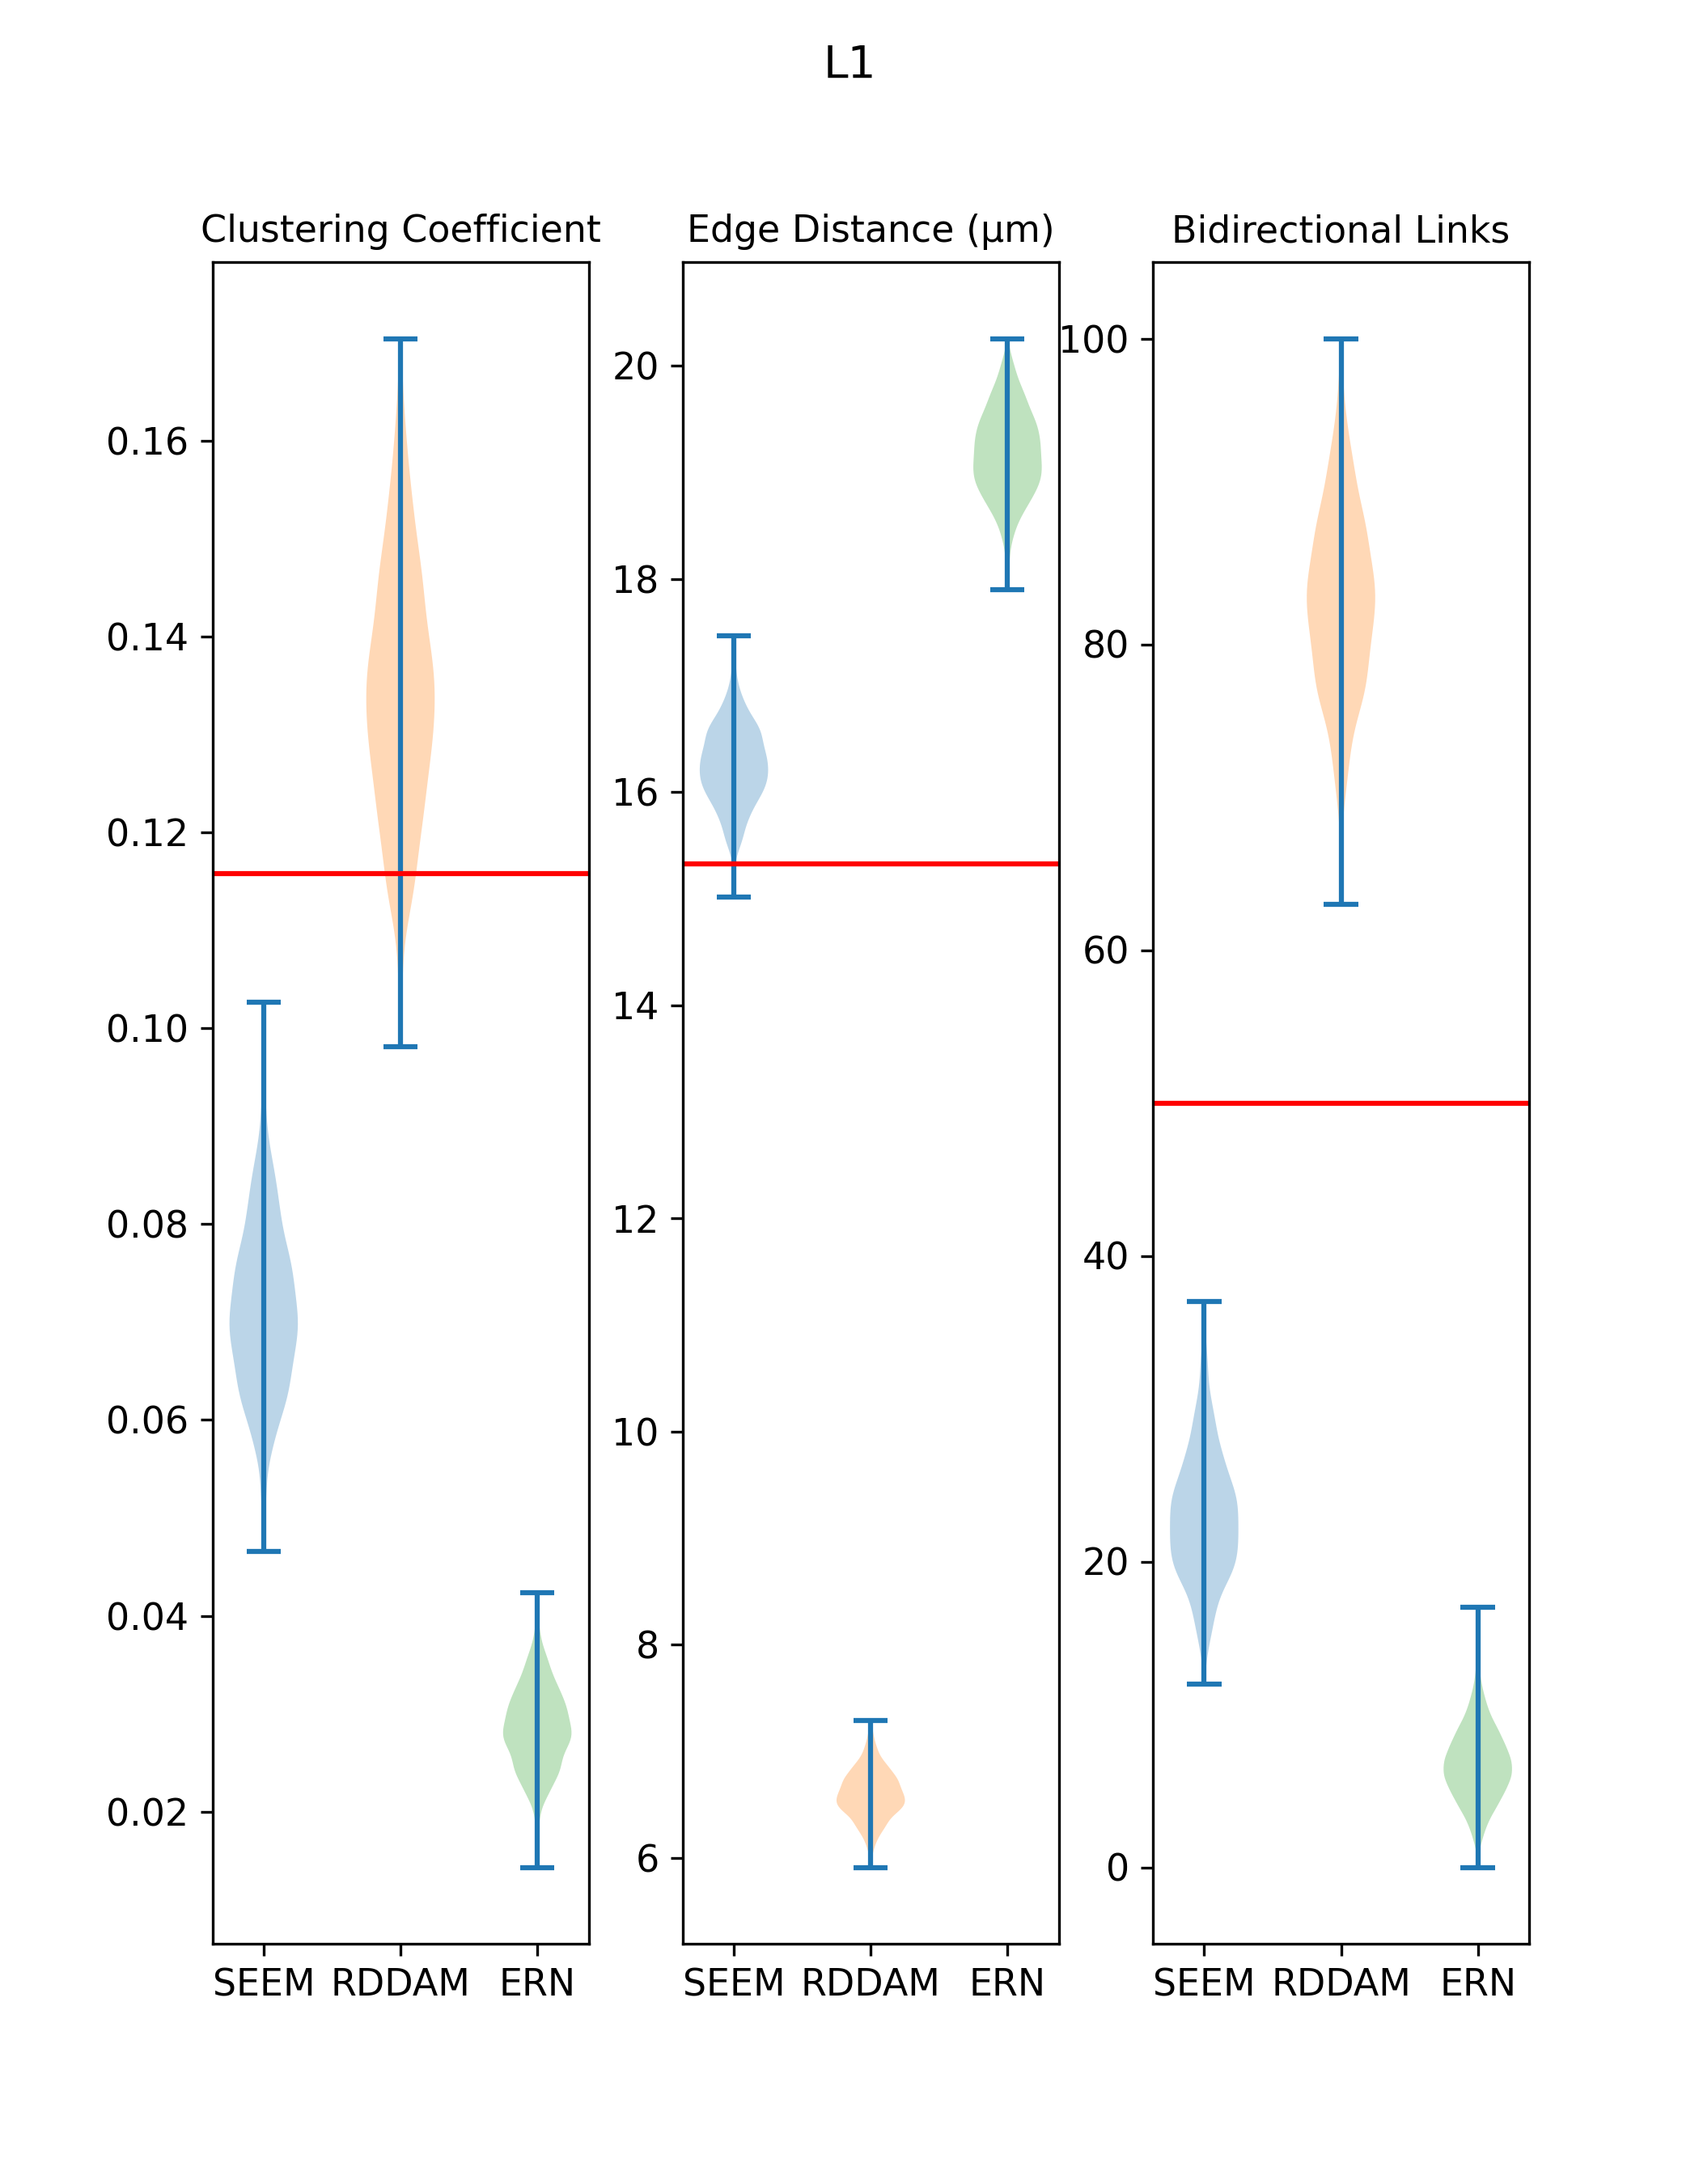
\includegraphics[width=0.49\linewidth]{../data/images/stats/L1.png}
  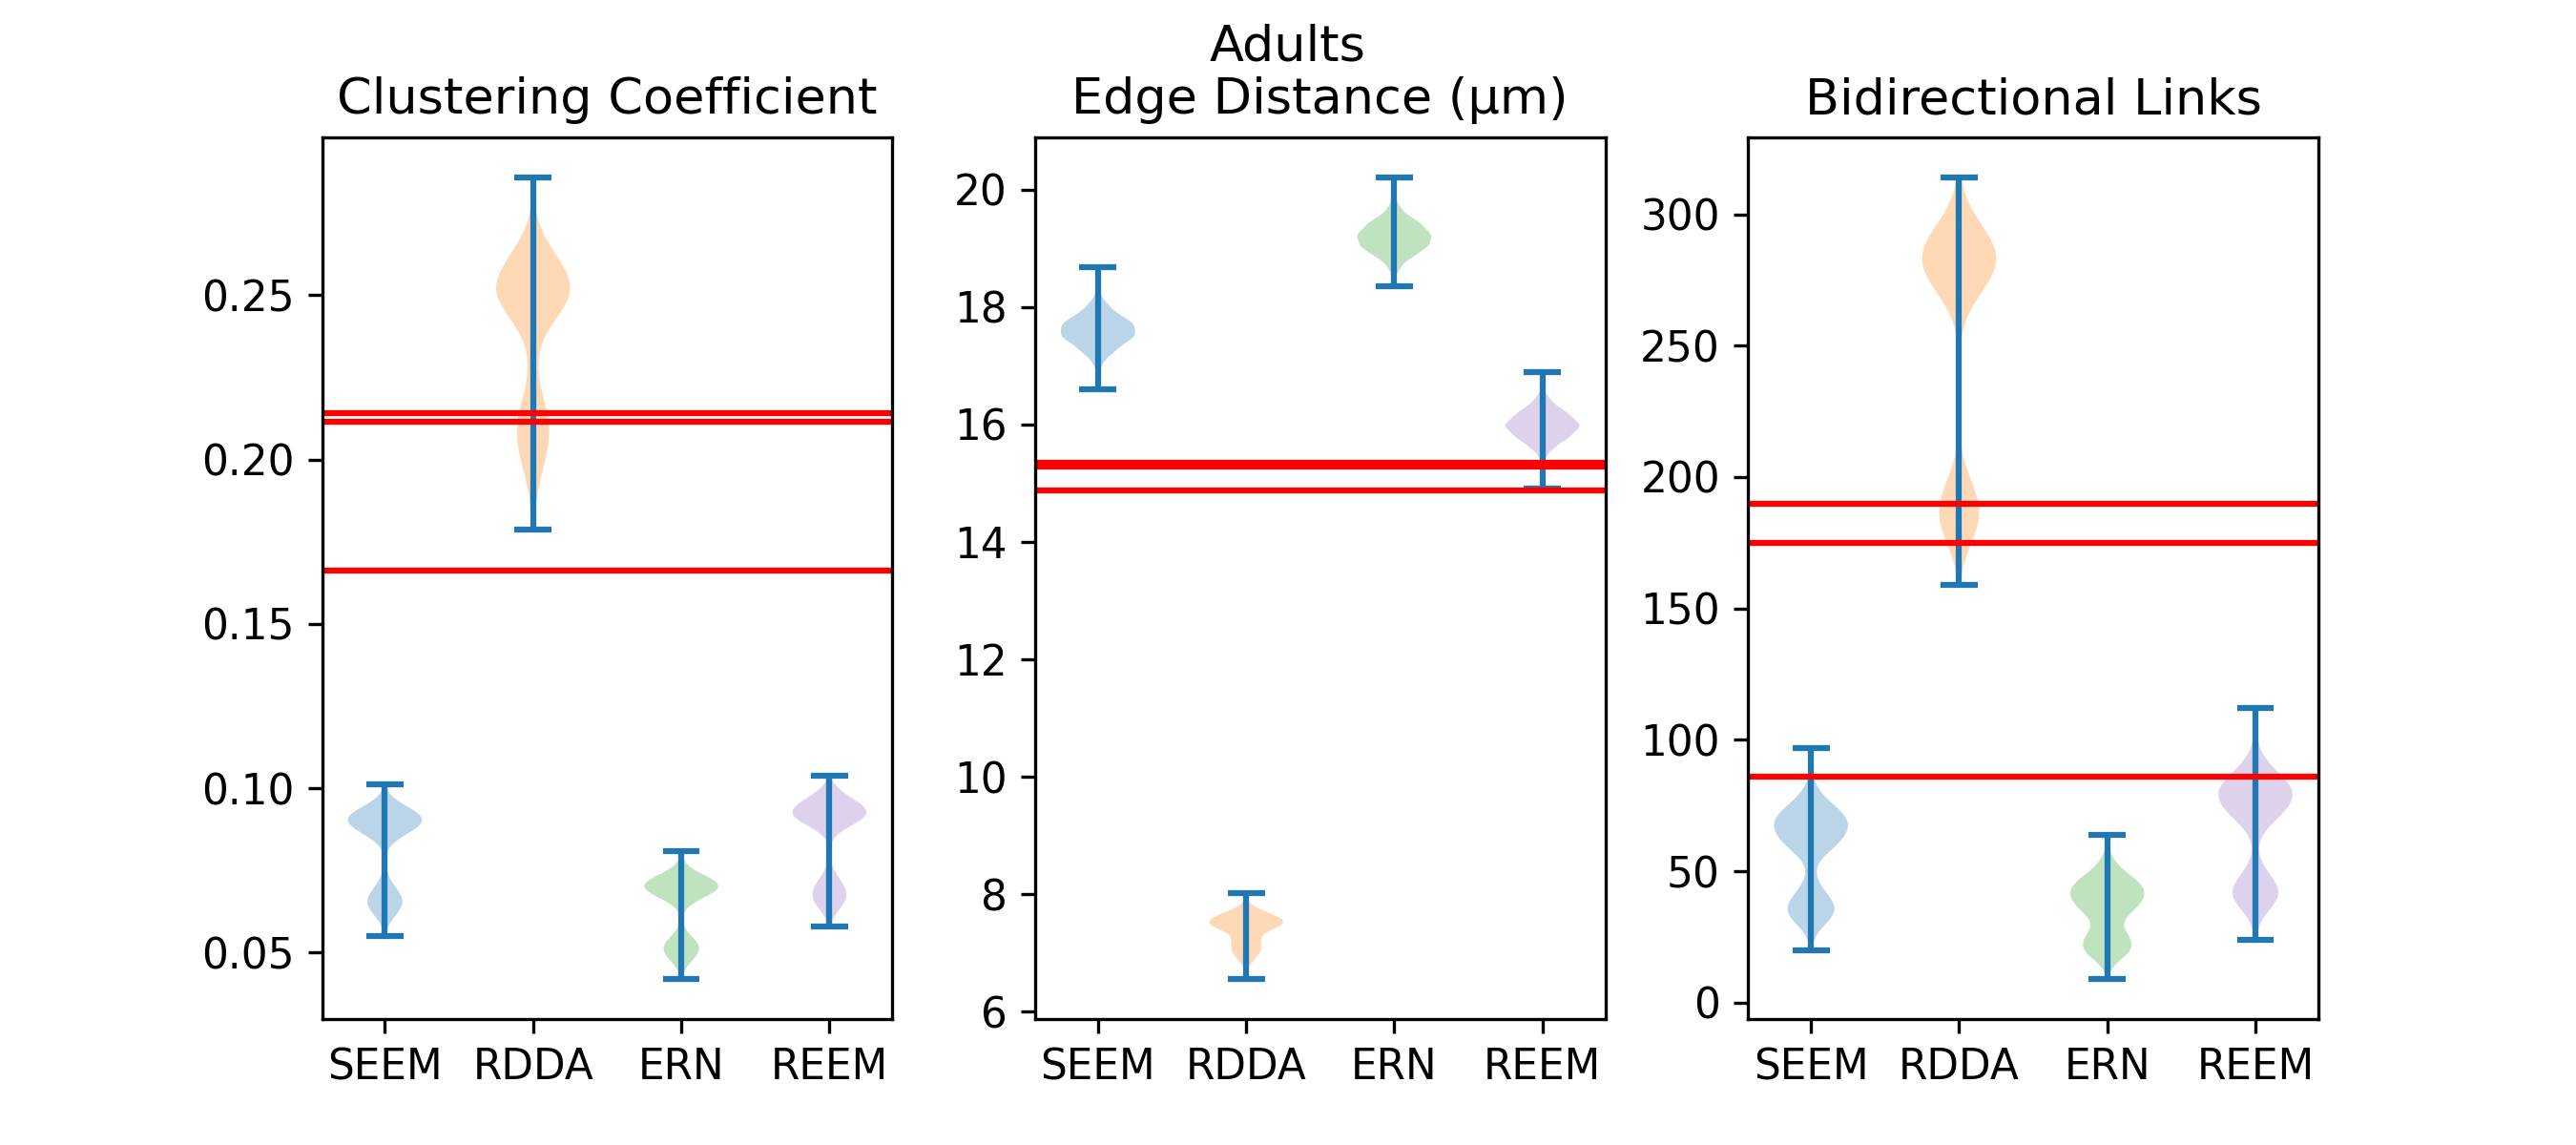
\includegraphics[width=0.49\linewidth]{../data/images/stats/Adults.png}
  \caption{INSERT HERE}
\end{figure*}

% \subsection{NOTES}
% The Results section is what needs the most work. It’s not clear yet what the Results are and what we are learning from them. If there are three or four sections to the Results — each section should be clearly titled.  I see a table and three figures — are each of those meant to be one of the sections of the Results? 
% Each figure should have a caption. The caption should start with a title: what is it about, the big picture. Then the details of what it is that we are looking at. The text in the section that corresponds to it should dive deeper. Each section should answer four questions:
% 1. Why are we doing this specific experiment. 
% 2. What is the experiment and how are we going about it. 
% 3. What is the observation of the results in detail.
% 4. What is the interpretation, what do we take away from the experiment. 

\subsection{Initial Model}

To answer the question of whether spatially embedding edges is an important factor in the formation of the \textit{C. elegans} Neural Network (CENN), we compared networks from SEEM with the CENN. In order to gauge how close our model is to the \textit{C. elegans} networks, we also compared these networks with RDDAM and random networks (Erdos-Renyi Networks / ERN). To rule out development as a factor, we made comparisons to both a single L1 connectome (~0 hours) and a set of 3 adult (L5) connectomes (INSERT REFERENCE). We measured these generative network models from a set of 1000.

NOTE: Is it clear that we are averaging across 1000 graphs?

\subsubsection{Network Statistics}
Comparing these networks can be done in several different ways. As an initial comparison, we chose to use network statistics to compare essential aspects of these graphs. 

We chose to compare the average clustering coefficient, average edge distance, and average total number of bidirectional links. These network statistics were chosen as they were used by Itzhack \& Louzoun (2010) in their paper on the RDDAM. 

We plotted the results of the network measures of all 1000 instances of each model (see fig 1) and compared them with the results of these measures on the CENN. For the newborn (L1), we compared it to a single graph, but, for the adults (L5), this was three graphs.

% 3. What is the observation of the results in detail.
% 4. What is the interpretation, what do we take away from the experiment. 

Looking at the results, we did not notice a significant difference between the results of L1 and L5 networks. One difference of interest was that the networks of Witvliet et al. (2021) had noticeably different clustering coefficients and total number of bidirectional links when compared with the enhanced connectome of White et al. (1984) (NOTE: N2U). It is difficult to determine what might be causing this discrepancy, whether it is a result of different environmental conditions or if this is indicative of flaws in recording methods of some or all of the connectomes. Rather than averaging the results of the connectomes, we chose to show all three individually (see fig 1). 

\begin{table}[h]
  \import{}{../data/spreadsheets/data}
  \caption{INSERT HERE}
\end{table}

\textit{Clustering Coefficient:} RDDAM was closest to \ce in this statistic. This reinforces the idea that spatial proximity plays an important role in how neurons form connections and how they cluster in the way they do. It is surprising that our model did not have a stronger clustering coefficient given that closer neurites do not need to cross as large of a distance to potentially connect. This might account for why our model does slightly better than a random network. Although this difference is not that great.

\textit{Edge Distance:} The average edge distance found that our model was the closest to \ce in this regard. It is important to note that our random networks were not that far behind. RDDAM had much shorter edges on average than any of the other networks. Given that it prioritizes proximity when making connections, this result is unsurprising. Given that our model was most similar to \ce in edge distance, this suggests that spatial embedding of neurites and soma alone might explain this characteristic of the network. As explained in the last section, neurites that start close to each other would be more likely to cross paths than those that start far away from each other.

\textit{Bidirectional Links:} The number of bidirectional links in \ce do not appear to be similar to any of the graphs resultant of these presented models. Given that our model creates graphs which are random subgraphs of a bidirectional set of all potential connections, directionality does not play a role in deciding connections. It having a higher number of bidirectional links can simply be explained by this reduced pool of connections to pick from. One is more likely to flip two heads with a coin than one is to roll two 1's with a die, given the same number of flips/rolls. By the same logic, a marginal increase in the number of bidirectional links likely is not a result of any novel network property.
The RDDAM overrepresents bidirectional links. Given its preference for short connections, an even smaller subset of possible connections are most likely to be made, which are direction agnostic. This would explain why RDDAM has so many bidirectional links. The stochasticity of the model would also explain the larger range of values. None of these models sufficiently explain the amount of bidirectional links exhibited by \ce. 

% NOTE: Look at the distribution of bidirectional links along edge distance. What does \ce look like?

% NOTE: Take a second look at the final measure and try to replicate.

% NOTE: Measure centrality??

\textit{What does this tell us?} Looking at these statistics, it appears that RDDAM well characterizes the highly clustered neuronal networks of \ce. The edge distance of \ce appears to be only slightly shorter than random, which is likely explained by the spatial embedding of the network. The bidirectionality of \ce could not be explained by any network. 
It is notable that for all of these measures the results of our model are similar to random networks. This might be a result of how instance networks are created through random selection. It might also indicate that this network is not selective enough. As it stands, there is not a definitive explanation for these results.

\begin{figure*}[h]
    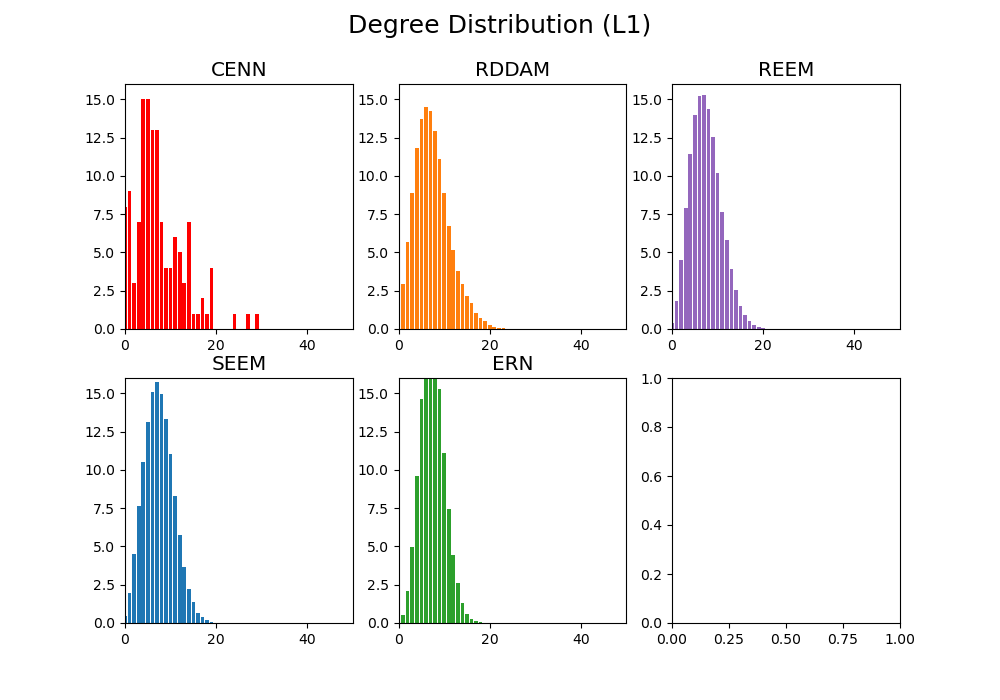
\includegraphics[width=0.32\linewidth]{../data/images/distributions/degreeDist_W1_Rand.png}
    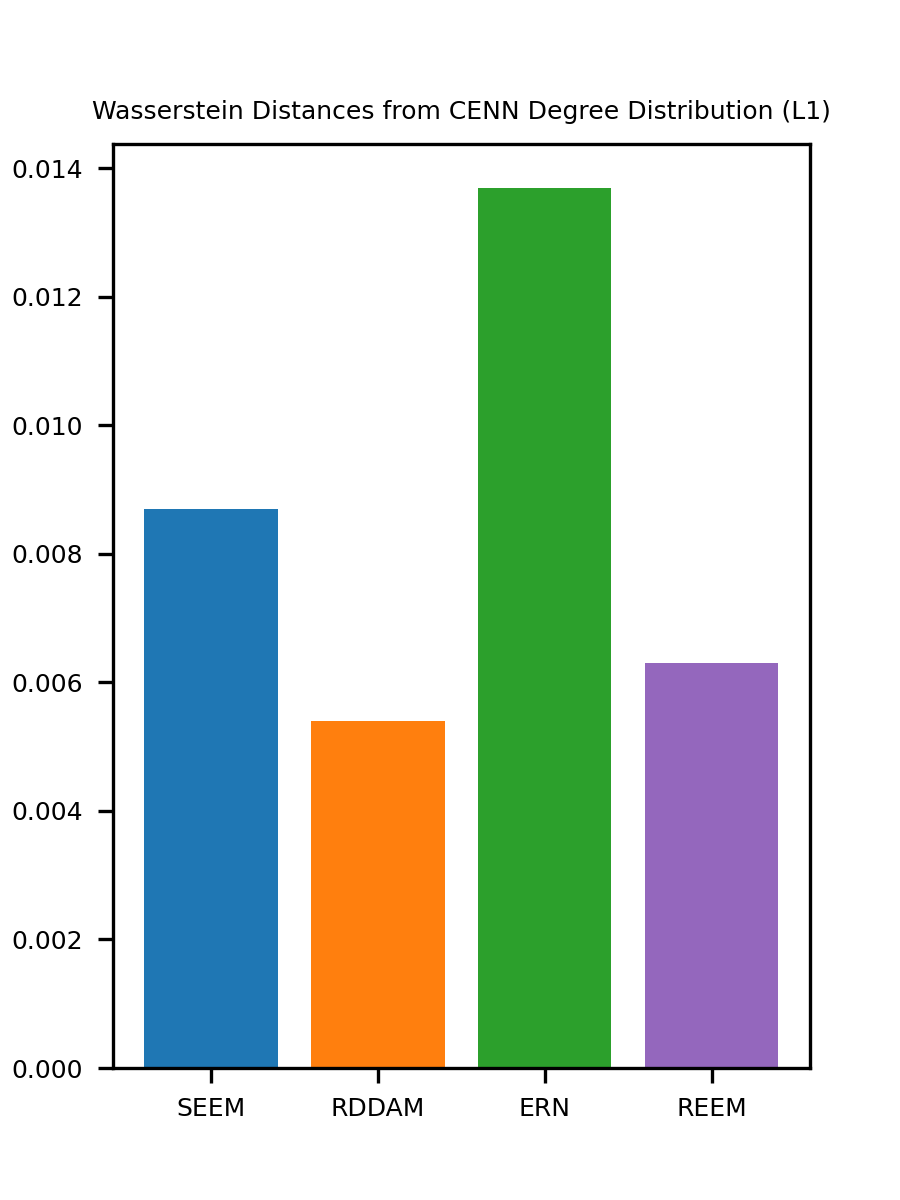
\includegraphics[width=0.17\linewidth]{../data/images/compareDistributions/wassersteinDistances_Degree_L1_3.png}
    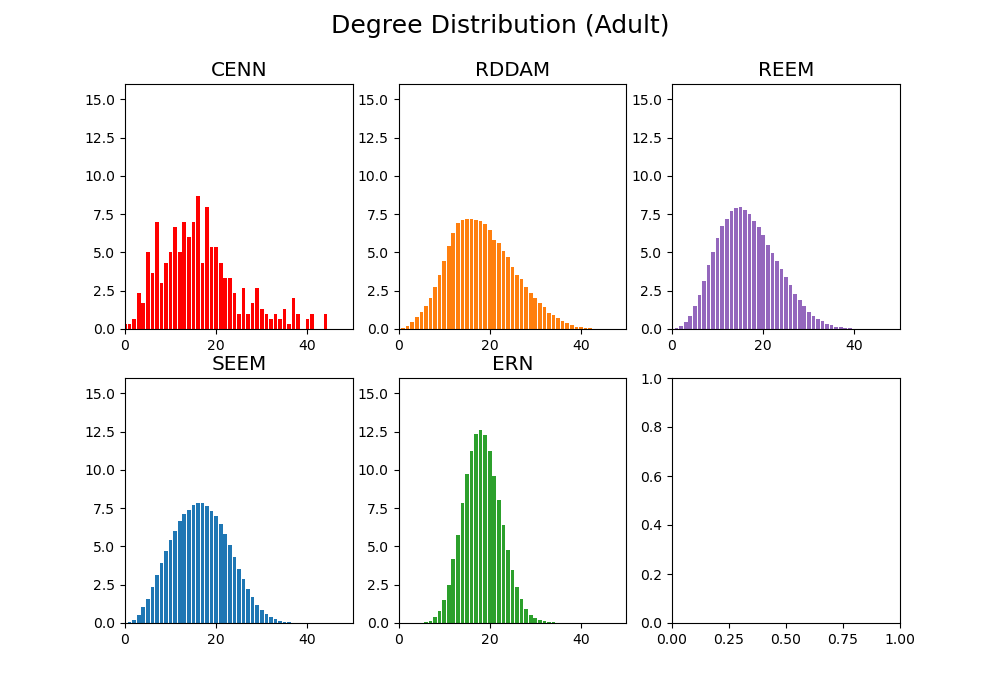
\includegraphics[width=0.32\linewidth]{../data/images/distributions/degreeDist_L5_Rand.png}
    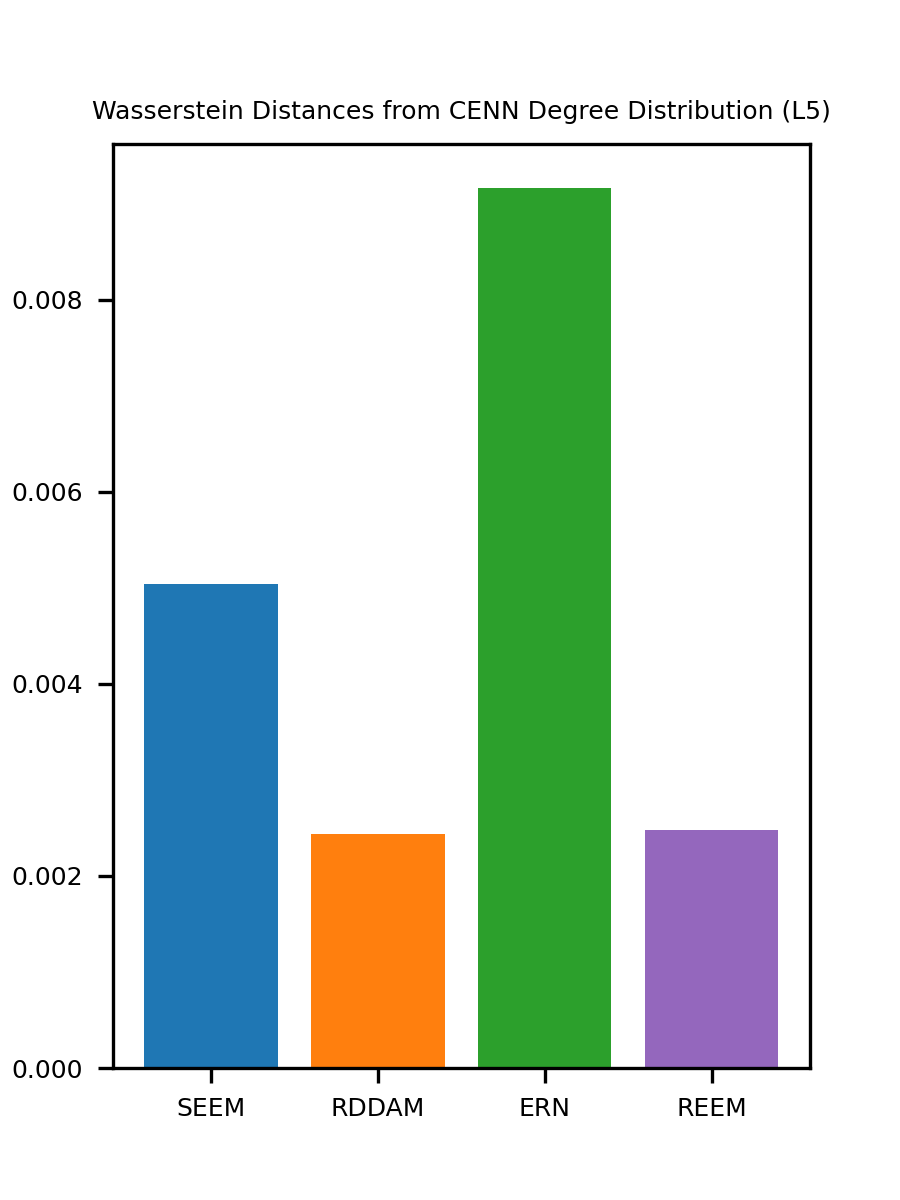
\includegraphics[width=0.17\linewidth]{../data/images/compareDistributions/wassersteinDistances_Degree_L5_3.png}

    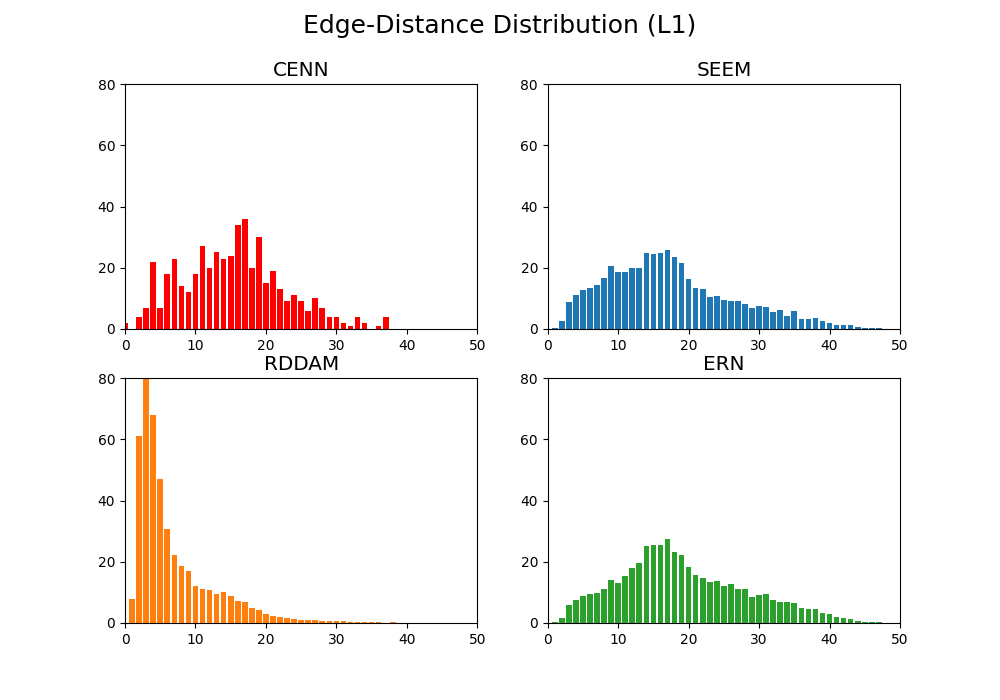
\includegraphics[width=0.32\linewidth]{../data/images/distributions/distDist_W1.png}
    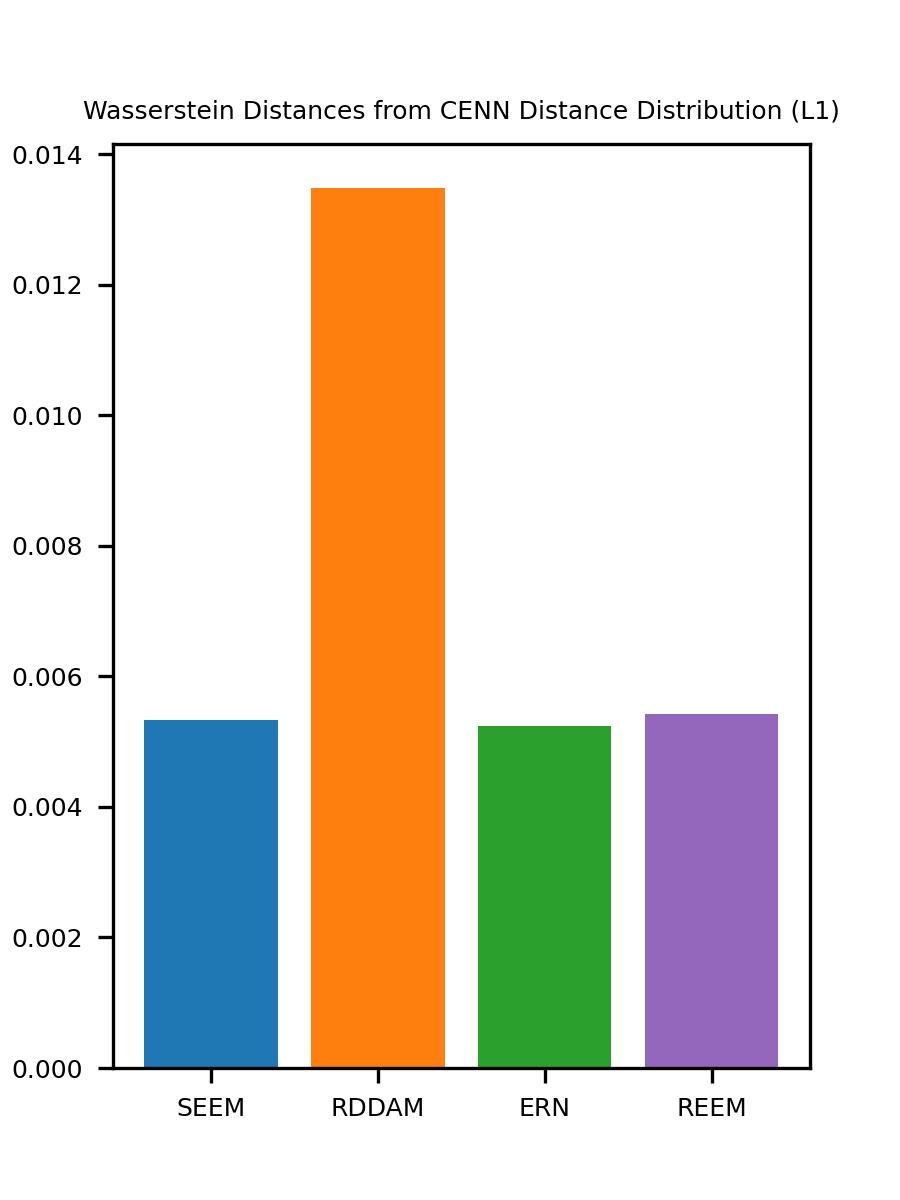
\includegraphics[width=0.17\linewidth]{../data/images/compareDistributions/wassersteinDistances_Distance_L1_3.png}
    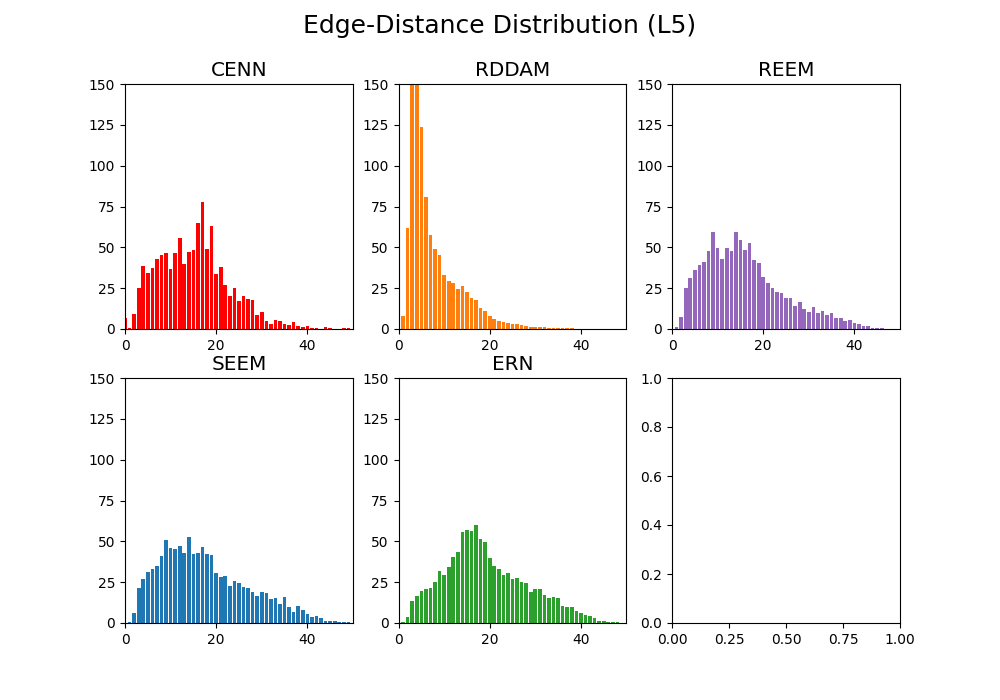
\includegraphics[width=0.32\linewidth]{../data/images/distributions/distDist_W8.png}
    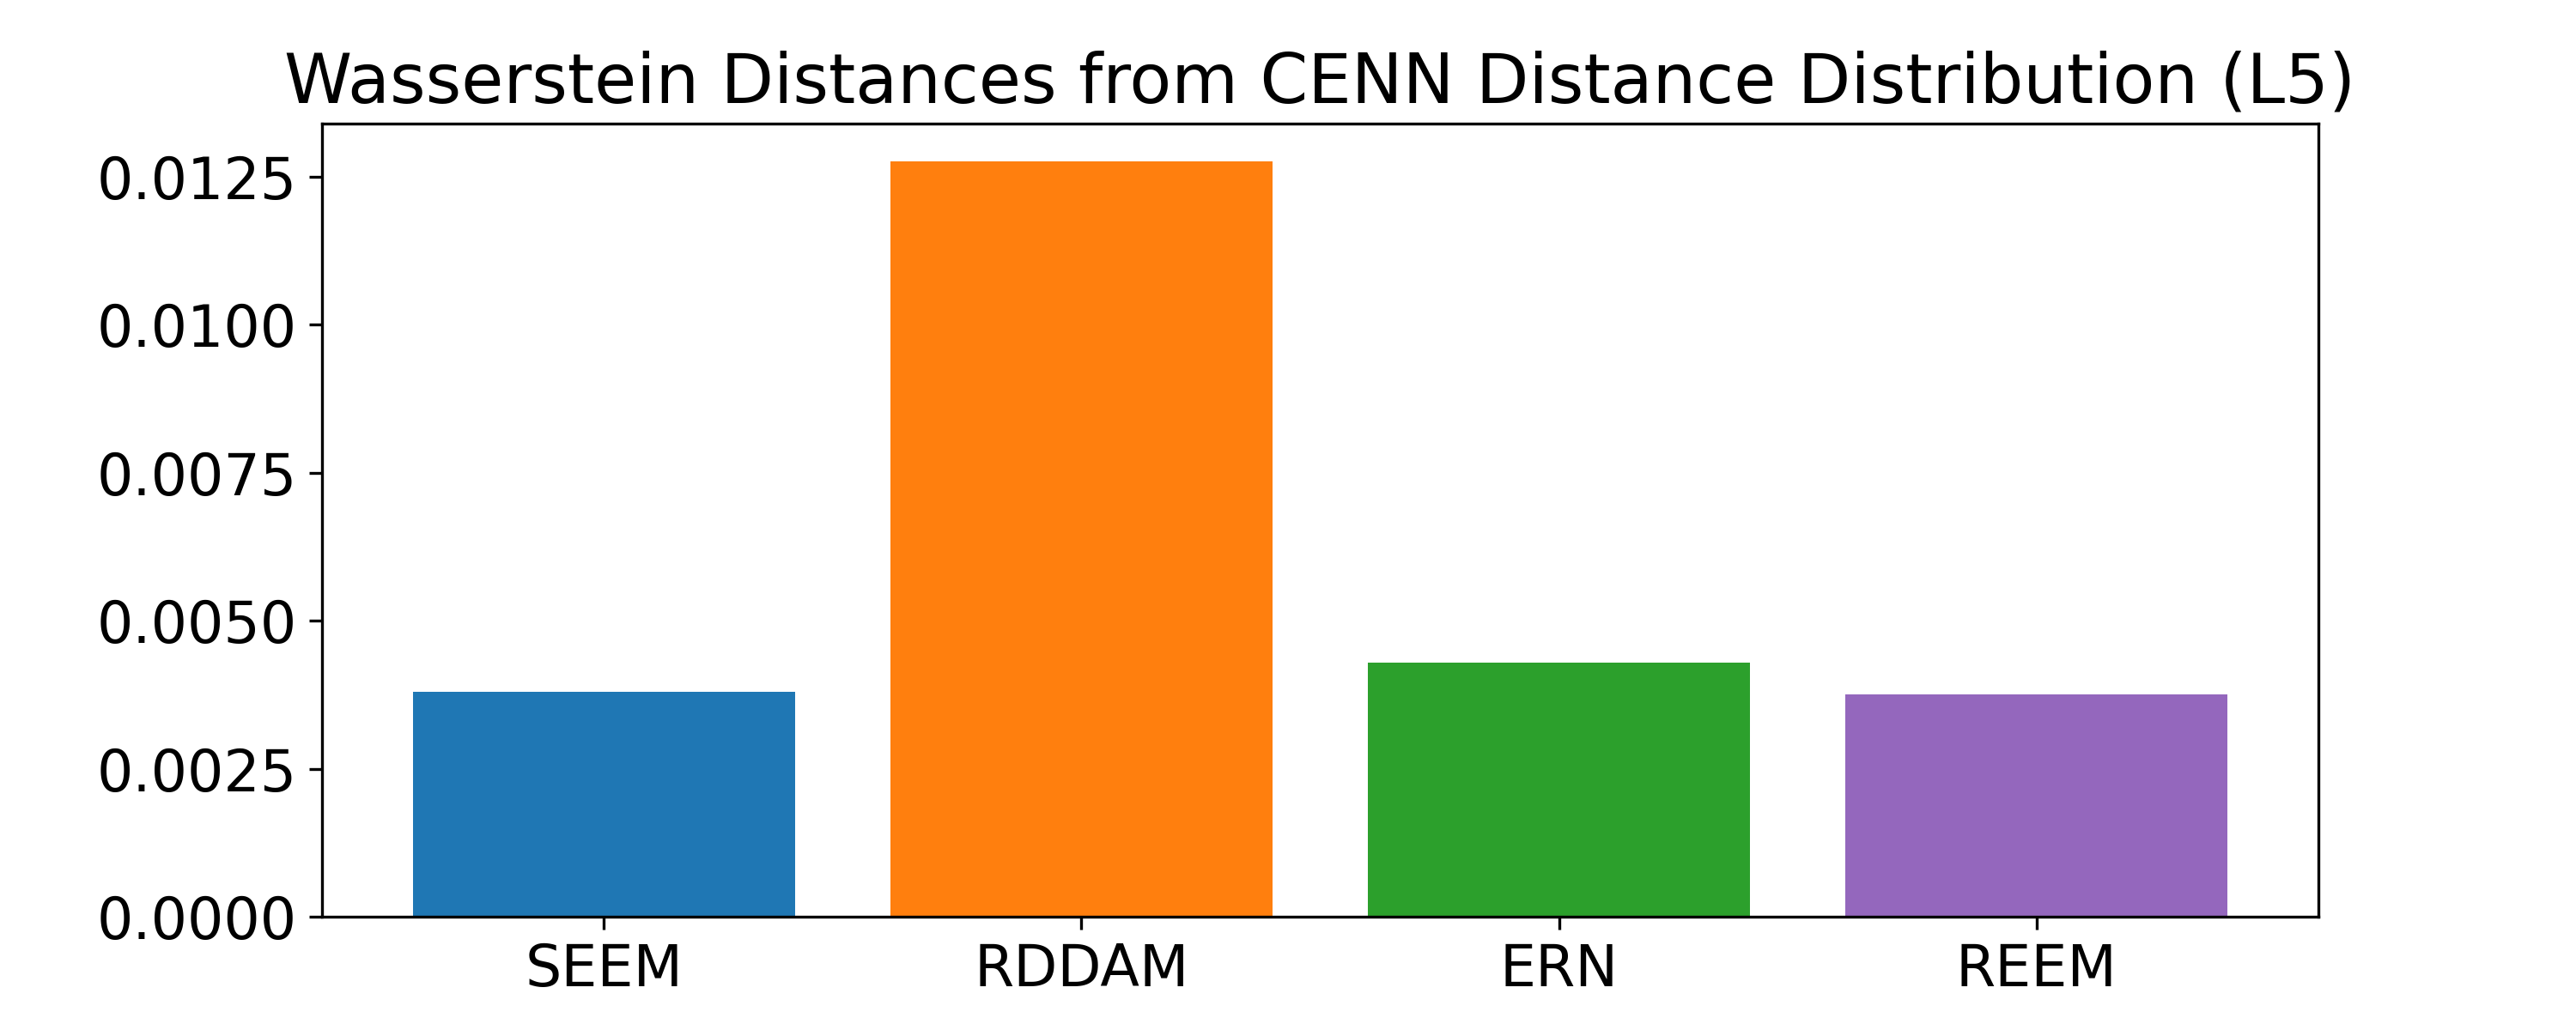
\includegraphics[width=0.17\linewidth]{../data/images/compareDistributions/wassersteinDistances_Distance_L5_3.png}

    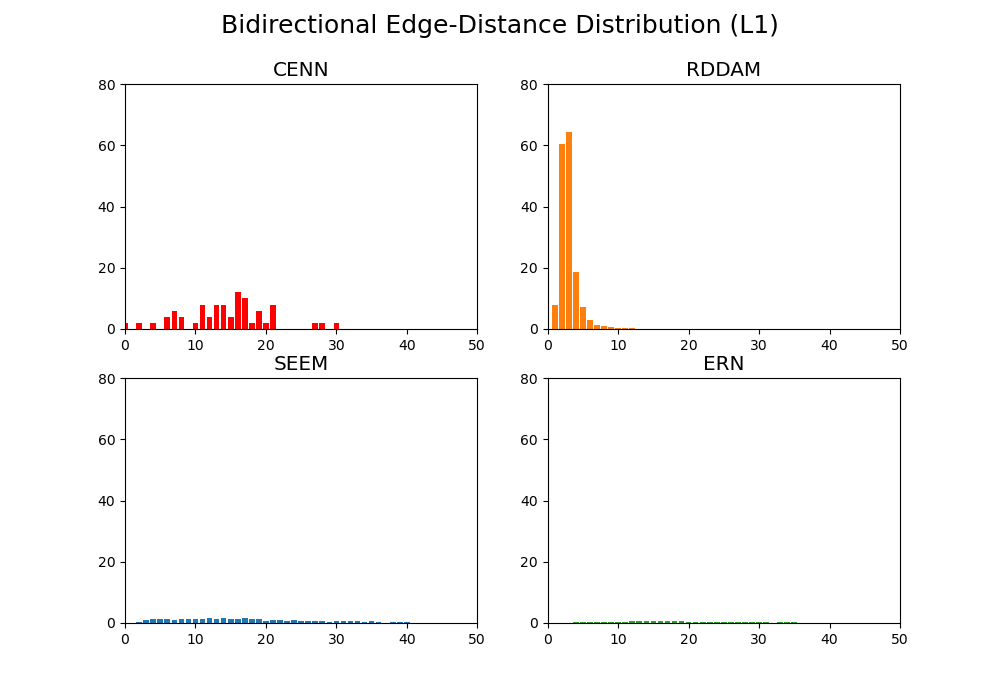
\includegraphics[width=0.32\linewidth]{../data/images/distributions/bidistDist_W1.png}
    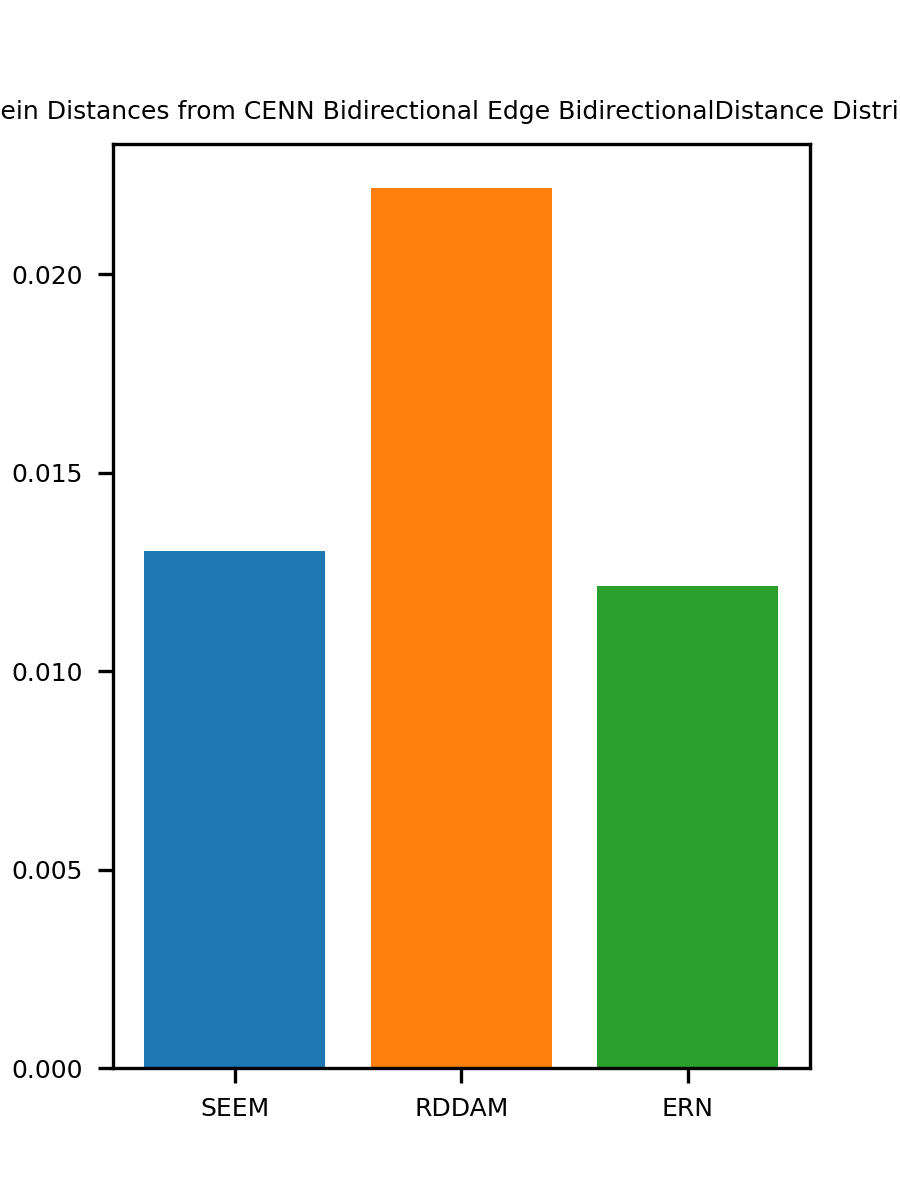
\includegraphics[width=0.17\linewidth]{../data/images/compareDistributions/wassersteinDistances_BidirectionalDistance_L1_3.png}
    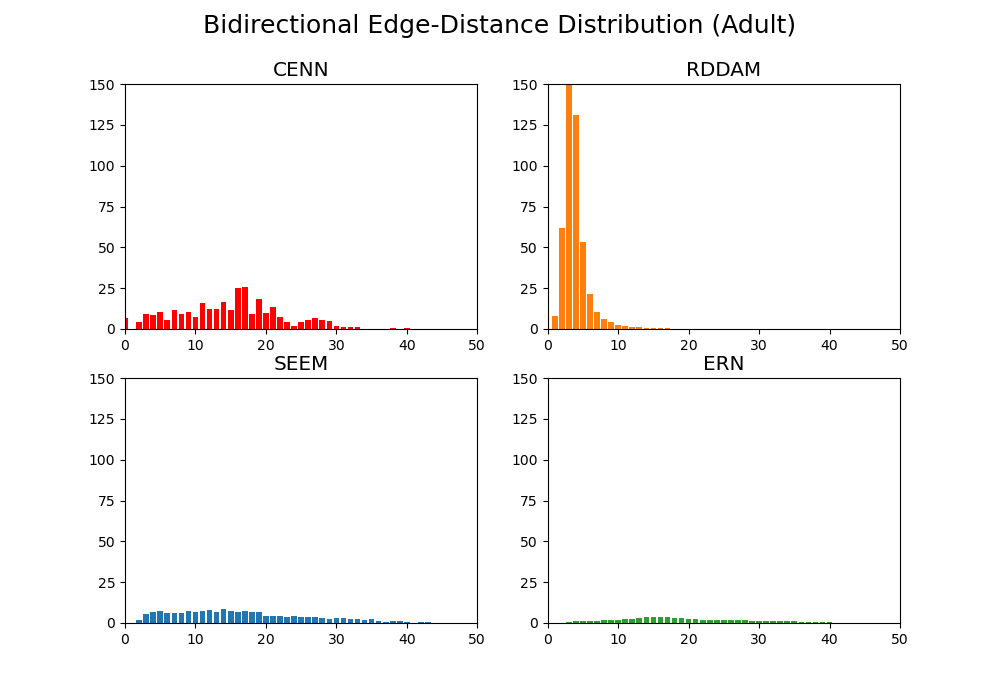
\includegraphics[width=0.32\linewidth]{../data/images/distributions/bidistDist_W8.png}
    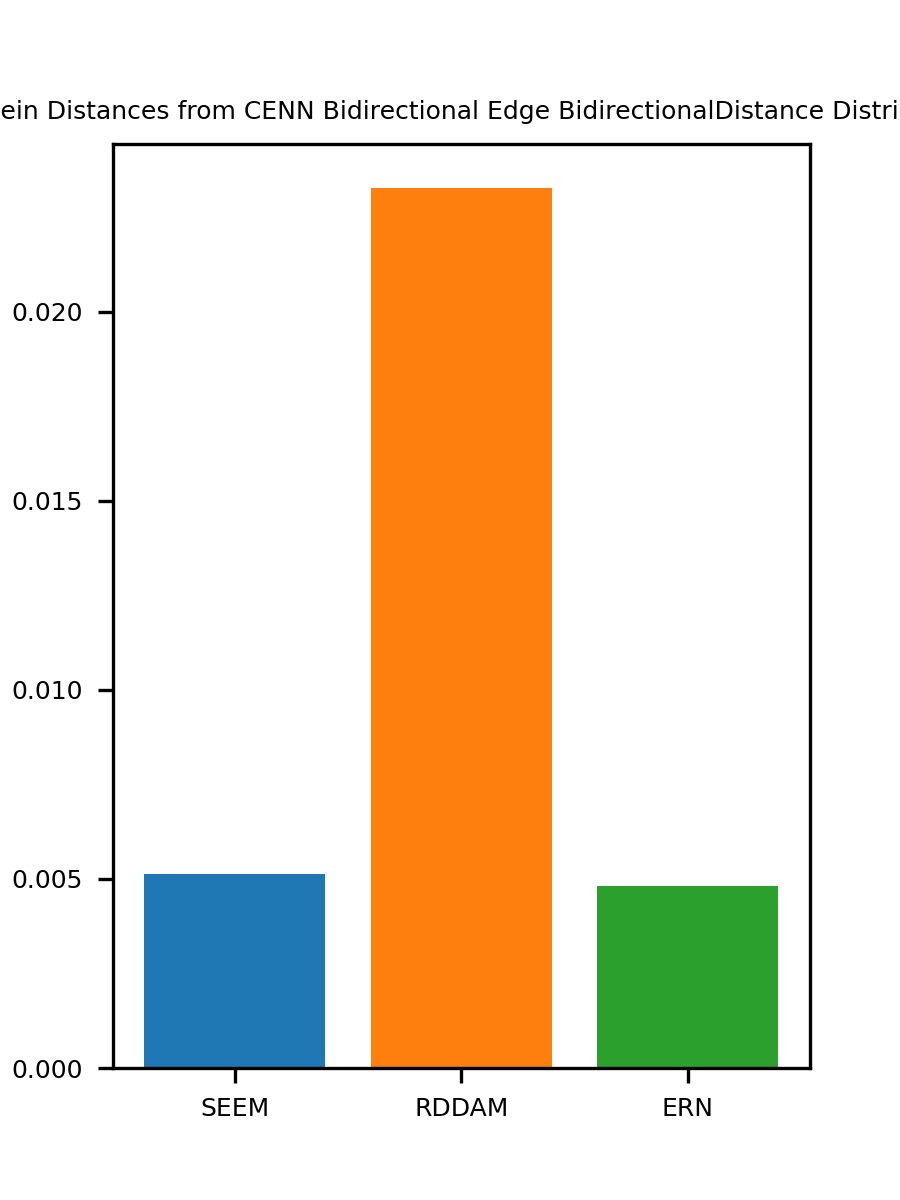
\includegraphics[width=0.17\linewidth]{../data/images/compareDistributions/wassersteinDistances_BidirectionalDistance_L5_3.png}

  \caption{Degree distributions, plotting the number of nodes (y-axis) with a particular number of connections (x-axis). \textbf{NOTE:} Going to remove the purple sections from these graphs, use line graphs so I can overlap all distributions, add more caption, add letter labels, and will likely seperate and improve the bottom two graphs. }
\end{figure*}

\subsubsection{Distributions}

While these statistics give us an idea of how some of the attributes of these networks in describing the underlying structure of the CENN, it does not give us a picture of how the edges in any of these networks are distributed. We had two questions: 1) What is the structural makeup of these networks? (Are they scale-free, small-world, etc.?) 2) What is the physical makeup of these networks?

To answer these questions, we compared the degree distributions of these networks to examine their network structure and the distance distributions of these networks to examine their physical structure (see fig 2). To get a better idea of how similar these distributions were, we also measured their Wasserstein Distances from the \ce distribution. For the adults, these distributions were averaged.

\textit{Degree Distributions:} We found that our model and RDDAM to have degree distributions closest to \ce, with RDDAM being slightly closer. This is the first result which differentiates our model from random networks. These two models result in networks which appear to have more variability in degree than random networks. Since both rely on spatial proximity of nodes, which are not evenly distributed, it would be expected for their degree distributions to favor nodes which are closer to many others. This could explain why we see these results. It is notable that the degree distributions of CENN have much longer tales. This means that \ce connectomes are more centralized than any of the other networks being compared.

\textit{Distance Distributions:} The edge distances of each model show an issue with RDDAM: it favoring close connections. We see that our model is most like \ce in this distribution, the same as what we found when comparing average edge distributions. This indicates that \ce frontal ganglia is not particularly distance dependent as indicated in Itzhack \& Louzoun (2010). Given the similarity in the distributions, spatial embedding alone could explain for the edge distance distribution of \ce. 

\textit{Bidirectional Edges:} Given the results of comparing numbers of bidirectional edges in these networks, we were curious as to what these bidirectional connections looked like in \ce. Did they result from a preference for short connections, were they random, or were they distributed in a completely different way from any of our models. To answer this, we compared the edge distance distributions of all bidirectional edges in each graph (see fig 2). From the results, the bidirectionality of \ce frontal ganglia appears to be mostly random with the random graphs being closest to \ce and our model being a close second. RDDAM, preferring short connections, resulting in a very different looking distribution. Despite the number of bidirectional edges being between the amount shown in RDDAM and our model, it appears that these connections are random with respect to spatial distance. It is important to note that the number of bidirectional edges is still much higher than one would expect in a random graph. 

% \textbf{NOTE:} I need to reexamine the source data to understand if these connections are electric or chemical. Shouldn't we expect the majority of connections to be bidirectional since most are electrical? Is there a misinterepretation of the data?

\begin{figure*}[h]
  \includegraphics[width=\linewidth]{../data/images/other/SpatialOverlaps.png}
  \caption{INSERT HERE}
\end{figure*}

\subsubsection{Spatial Embedding}
\subsubsection{Overlaps}

\subsection{Breaking Down the Model}
What aspects of SEEM lead to a model that in some ways is more similar to the CENN? This model's input parameters are the location of the neurons, the expected number of connections, the location of the Nerve Ring (VALUE), and Epsilon (the maximum distance two neurites must have to form a potential connection. The first two of these parameters come from empirical data so they will not be adjusted. Adjustment of the location of the Nerve Ring cannot be meaningfully adjusted as there are only a small number of neurons which closely lie on this border, making such changes insignificantly impactful to the overall shape of the network. Rather than adjusting the nerve ring location, adjusting the algorithm for determining neurite direction may prove as more useful in parsing out the model's relavent parameters. 

\textbf{THIS IS WHERE WE TALK ABOUT THE RANDOM DIRECTION VERSION OF SEEM.}

% \subsection{Neurite Direction}
% Is neurite direction a significant factor in forming models which are similar to the CENN?

% \subsection{Attachment Distance}
% Is the maximum attachment distance between neurites important for creating a network more similar to the CENN?

% \section{OLD}
% \subsection{Network Statistics CHANGE}
% SEEM was found to be the set of networks closest to the CENN in average edge distance (see table 1 and fig 1). [INSERT STATS FOR STATISTICAL SIGNIFICANCE BETWEEN DISTRIBUTIONS]. RDDAM were closest to the CENN in average clustering coefficient and number of bidirectional links. [INSERT STATS FOR STATISTICAL SIGNIFICANCE BETWEEN DISTRIBUTIONS]. These results were not heavily dependent on which network was chosen.

% The degree distributions of RDDAM were also found to be most similar to the CENN with a Wasserstein Distance of 0.005 in L1 and 0.002 in adults (see fig 2). SEEM was close with a Wasserstein Distance of 0.006 in L1 and 0.003 in adults, making the distinction between the two insignificant. The degree distributions of Erdos-Renyi graphs appeared much less like the CENN with a Wasserstein Distance of 0.013 in L1 and 0.009 in adults. The average degree between all four graphs were not significantly different.




% Comparing the distribution of edge distances shows a different picture. Here, the resulting graphs of SEEM were found to be closest to the CENN (see fig 3). The edge distance distributions in SEEM had a Wasserstein Distance of 0.004 in L1 and 0.003 in adults. The Erdos-Renyi graphs, with a Wasserstein Distance of 0.005 in L1 and 0.004 in adults, were even more similar to CENN than the RDDAM, with a Wasserstein Distance of 0.013 in L1 and adults. These results distinguish SEEM from RDDAM, showing the proclivity of RDDAM to form very short connections, something SEEM does not appear to do.

% Spatially embedding these graphs using provided coordinates resulted in a particular connectivity pattern shared between the CENN and SEEM graphs (see Figure 4). [INSERT DATA ABOUT DISTRIBUTION OF CROSS-PHARYNX CONNECTIONS]